\section{Obtenção dos dados pluviométricos}

Os dados pluviográficos utilizados no presente trabalho foram fornecidos pela Unidade de Monitoramento da Rede Hidrometeorológica (UMR) que faz parte do Instituto de Tecnologia de Pernambuco (ITEP). O arquivo cedido, mostrado na Figura \ref{fig:arquivo}, contém dados pluviográficos, registrados entre os anos de 2000 e 2013, da plataforma de coleta de dados da cidade de Recife. Após exame do arquivo fornecido, não foram utilizados os anos em que ocorreu falha nos registros de precipitação, dessa maneira, foi escolhida uma serie histórica entre 2003 e 2011.

O arquivo contém registros de data e hora para cada incremento de precipitação de $0,25mm$ de chuva acumulada. Os dados foram separados por ano, uma vez que a sequência temporal é essencial para identificação dos intervalos de tempo entre as precipitações.

%Para obtenção das máximas precipitações diárias, verificou-se em todo arquivo a máxima precipitação anual ocorrida em cada intervalo de duração. Nesse estudo as durações adoradas foram: 5, 10, 15, 30, 60 120, 240, 360, 720 e 1080 minutos, em que as precipitações excedam 8, 10, 15, 20, 25, 30 33, 40, 47 e 55mm, respectivamente. 

Após obtenção dos dados do ITEP, foi realizada uma verificação para coleta de precipitações máximas diárias, por meio de um aplicativo matemático desenvolvido durante esse estudo, objetivando o estudo das chuvas intensas para obtenção das precipitações de máximas anuais e levando em conta os seguintes critérios:

\begin{enumerate}
    \item Foram utilizados períodos de retorno de 2, 5, 10, 15, 20, 25, 50 e 100 anos.
    \item Foram consideradas precipitações de chuvas intensas com durações de 5, 10, 20, 30, 60, 120, 180, 360, 720 e 1080 minutos que ultrapassam as alturas de 8, 10, 15, 20, 25, 30, 33, 40, 47 e 55mm, respectivamente.
    \item Duas ou mais chuvas acontecidas durante um intervalo de 24h são consideradas como uma única chuva.
    \item Foram analisadas todas as precipitações que apresentam altura pluviométrica superior a 15mm durante 24h.
\end{enumerate}

\begin{figure}[h]
    \caption{Formatação dos dados fornecido pelo ITEP para análise}
    \centering
    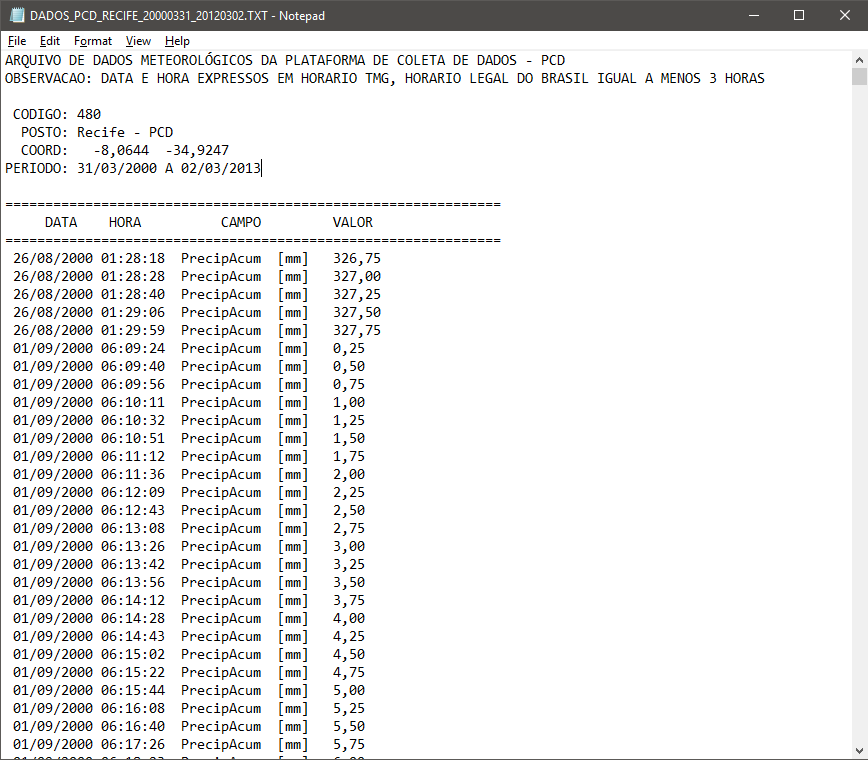
\includegraphics[width=0.8\textwidth]{Textuais/Figuras/arquivo.png}
    \fonte{Instituto de Tecnologia de Pernambuco (2013)}
    \label{fig:arquivo}
\end{figure}

Esses critérios foram adotados seguindo como modelo referências de \citeonline{hidro-basica}, \citeonline{hidro-aplicada} e \citeonline{tucci1993}.

\section{Determinação da equação IDF}

De acordo com \citeonline{hidro-aplicada}, deve-se analisar as relações entre intensidade-duração-frequência das chuvas, determinando para diferentes intervalos de duração, qual o tipo de equação e o número de parâmetros que melhor representam a região. A equação escolhida para esse projeto será a equação geral, representada pela Equação \ref{eq:equacao-geral}, devido a adoção por diversos autores.

Para obter as séries históricas de máximas precipitações, verificou-se, para a PCD escolhida, a máxima precipitação anual para cada intervalo de duração. A duração de 5 minutos, adotou-se, conforme os critérios comentados anteriormente.

Após a determinação das máximas precipitações anuais, será encontrada a melhor distribuição empírica de probabilidade que se ajuste aos dados.
Para realizar a extrapolação dos dados será utilizada a distribuição estatística para valores máximos extremos de Gumbel.

\subsection{Teste de aderência}

Será realizado um teste estatístico para validar se a distribuição adotada realmente representa os dados empíricos. Como comentado no capítulo anterior, em algumas regiões do Brasil não são comuns o monitoramento histórico de chuvas, sendo admissível a utilização de períodos inferiores ao recomendado mediante a alguns testes de validação. Dentre esses, o teste de Kolmogorov-Smirnov é utilizado para testar e validar o ajuste de distribuições contínuas.

\subsection{Obtenção dos parâmetros da equação IDF}

Nesse trabalho, para calcular os coeficientes k, a, b e c da Equação \ref{eq:equacao-geral}, foi adotada a metodologia de Regressão Linear Múltipla, desenvolvida na linguagem Python 3.2. Logaritimizando a Equação \ref{eq:equacao-geral}, obtem-se a Equação \ref{eq:eqcomlog}.

\begin{equation}
\label{eq:eqcomlog}
    log(i) = log(A) - c \times log(t+b)
\end{equation}

Onde

\begin{equation}
    \label{eq:loga}
    log(A) = log(k) + a \times log(T_r)
\end{equation}

A Equação \ref{eq:eqcomlog} é função de uma reta com coeficiente angular $c$ e coeficiente linear $log(A)$. Para estimativa do parâmetro $b$ foi aplicado uma variação dentro do intervalo de -100 a 100 que melhor transforma as curvas obtidas em uma reta, com intuito de obter um valor inicial de $b$. O valor de $b$, foi ajustado para um valor que proporciona o maior coeficiente de determinação da correção linear entre log(i) e log(t+b). O valor médio da constante $c$ é calculado por meio da média entre os valores encontrados em cada reta para cada período de retorno estudado nesse trabalho. Enquanto os valores de $log(A)$ servem para determinação das constantes $a$ e $k$.

A Equação \ref{eq:loga} é também uma equação de reta, com coeficiente angular $a$ e coeficiente linear $log(k)$. De modo análogo, os valores de $log(A)$, anteriormente obtidos, e $log(T_r)$ são correlacionados para determinação dos valores de $a$ e $k$ da reta de regressão.